A métrica para cálculo de desempenho dos modelos durante a competição no \emph{Kaggle} foi a acurácia, e o melhor resultado obtido na competição foi de 71.161\%. Os resultados de acurácia e \emph{F1 Micro} para os modelos de CNN testados, bem com o \emph{Ensemble} obtiveram os mesmos valores, visto isso é apresentado somente o valor da medida \emph{F}. Na Tabela \ref{tbl:fscore} observa-se os resultados para cada modelo de CNN, juntamento do resultado do \emph{Emsemble} das CNN com \emph{XGBoost}.

É observado que o melhor classificador, modelo 7, individual de CNN, obteve 69.49\% enquanto que o pior, modelo 9, obteve 62.44\%. Ressaltando que cada classificador de CNN usado no \emph{Ensemble} obteve resultados melhores do que os outros, em determinada expressão ou bons resultados em todas as expressões, mas não se sobressaiu em nenhuma expressão específica. No caso do modelo 9, obteve bons resultados em quase todas as expressões, mas não obteve-se nenhum resultado melhor na classificação de determinada expressão em relação aos outros modelos. Já no caso do modelo 7, obteve-se o melhor resultado de classificação para expressão de surpresa.

\begin{table}[!htb]
\centering
\caption{F1 Micro das Arquiteturas utilizadas}
\label{tbl:fscore}
\begin{tabular}{@{}cc@{}}
\toprule
Modelo & F1 Micro           \\ \midrule
1      & 0.6898857620507105 \\
2      & 0.6767901922541097 \\
3      & 0.6606297018668152 \\
4      & 0.6798551128448036 \\
5      & 0.6667595430482028 \\
6      & 0.6781833379771524 \\
7      & 0.694901086653664  \\
8      & 0.6285873502368348 \\
9      & 0.6244079130677069 \\ 
ensemble & 0.7174700473669546 \\ \bottomrule
\end{tabular}
\end{table}

As matrizes de confusão estão normalizadas. Cada célula foi colorida de acordo com a incidência de elementos contidos nesta antes da normalização(quanto maior a incidência mais escura é a cor da célula). O \emph{grid} de matrizes de confusões da Figura \ref{fig:grid} foi gerado a partir da parte \emph{PrivateTest} da base de dados, onde cada matriz corresponde a um modelo de CNN utilizado no \emph{Ensemble}. As classes verdadeiras do exemplo estão representadas pelas linhas, enquanto, as colunas representam as classes preditas pelo \emph{Ensemble}.

Na Figura \ref{fig:emsemble} é apresentado o resultado do modelo utilizando \emph{Ensemble}. Onde o resultado final de desempenho foi de 71.74\% de acordo com a métrica \emph{F1 Micro}, ressaltando que seu valor de Acurácia possui o mesmo valor. E com este resultado o \emph{Ensemble} supera, por pouco, o modelo campeão da competição.

\begin{figure}[!htb]
    \centering
    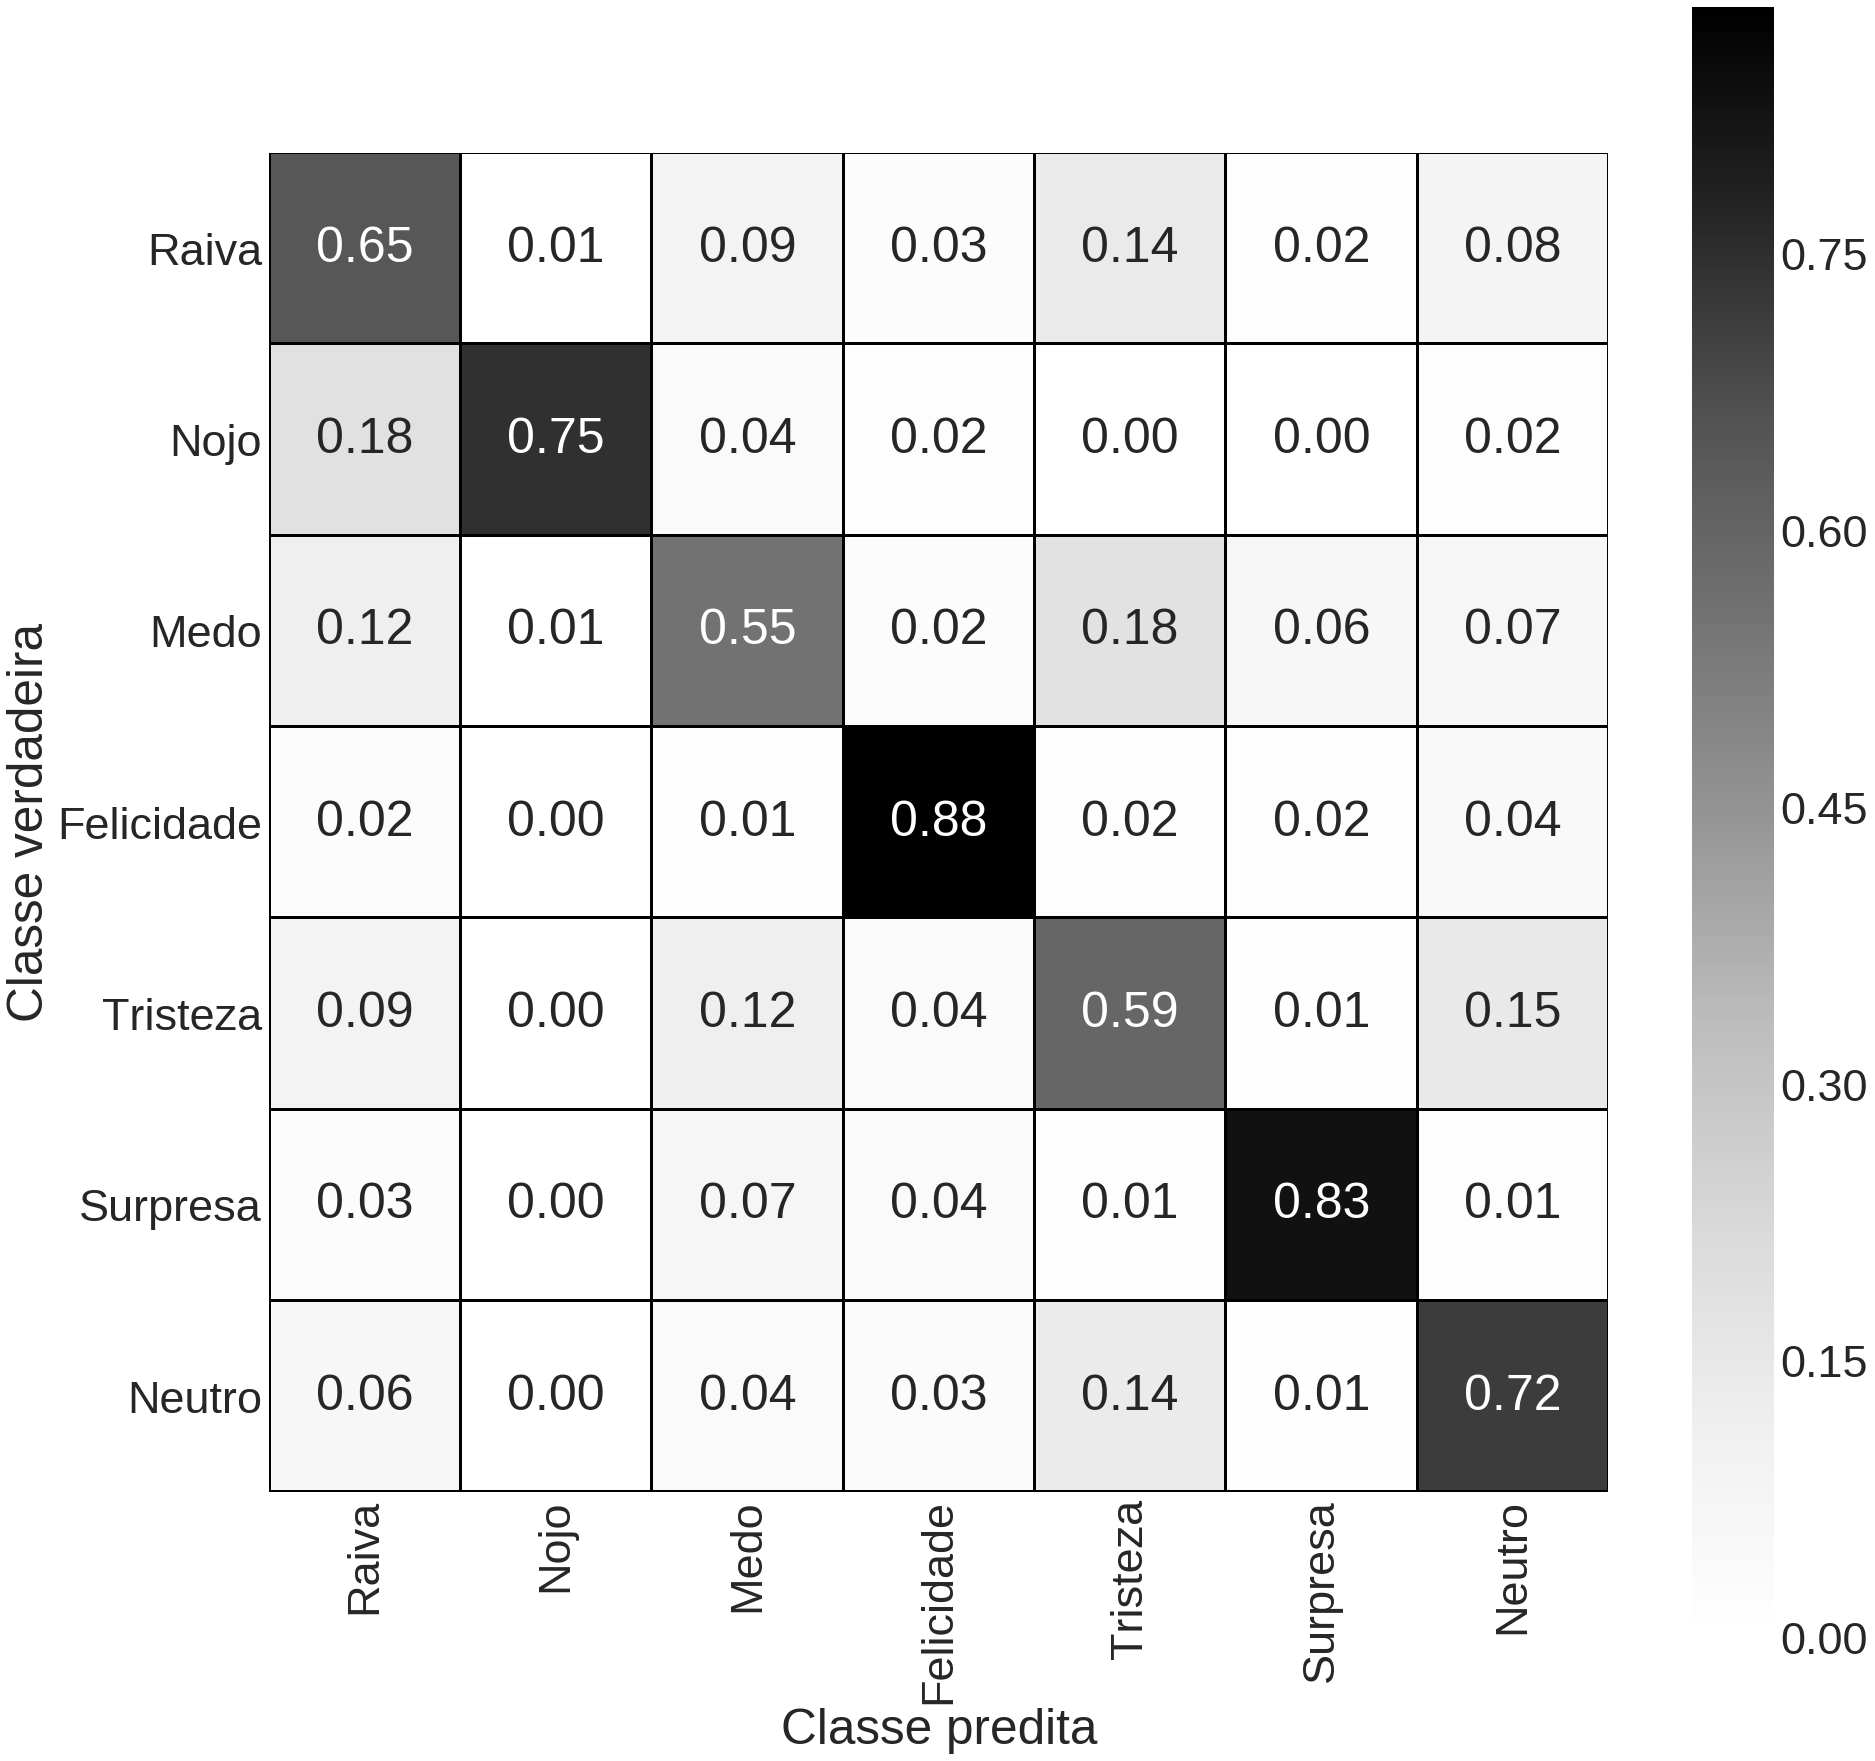
\includegraphics[width=7cm]{images/cm_emsemble.png}
    \caption{Matriz de Confusão do \emph{Emsemble} (CNN + \emph{XGBoost})}
    \label{fig:emsemble}
\end{figure}
